\documentclass[12pt,a4paper]{report}

% Packages
\usepackage[utf8]{inputenc}
\usepackage[T1]{fontenc}
\usepackage{amsmath}
\usepackage{amssymb}
\usepackage[lining]{ebgaramond}
\usepackage[cmintegrals,cmbraces]{newtxmath}
\usepackage{microtype}
\usepackage{geometry}
\usepackage{graphicx}
\usepackage{booktabs}
\usepackage{array}
\usepackage{xcolor}
\usepackage{hyperref}
\usepackage{float}
\usepackage{caption}
\usepackage{etoolbox}
\usepackage{enumitem}
\usepackage{makecell}
\graphicspath{{./fig/}}

% Page layout
\geometry{
    left=1.8cm,
    right=1.8cm,
    top=2.2cm,
    bottom=2.2cm
}

% Color definitions
\definecolor{crimson}{RGB}{153, 0, 0}

% Hyperlink settings
\hypersetup{
    colorlinks=true,
    linkcolor=crimson,
    urlcolor=crimson,
    citecolor=crimson
}

\tolerance=2000
\emergencystretch=2em

% Chapter/section title formatting
\usepackage{titlesec}
\titleformat{\chapter}{\normalfont\huge\bfseries}{}{0pt}{}[\vspace{0.3em}]
\titlespacing*{\chapter}{0pt}{0pt}{14pt}
\titleformat{\section}{\normalfont\Large\bfseries}{\thesection}{1em}{}
\titleformat{\subsection}{\normalfont\large\bfseries}{\thesubsection}{1em}{}

\setlength{\parindent}{0pt}
\setlength{\parskip}{4pt}

% Float spacing
\setlength{\floatsep}{6pt plus 2pt minus 2pt}
\setlength{\textfloatsep}{10pt plus 2pt minus 2pt}
\setlength{\intextsep}{10pt plus 2pt minus 2pt}
\setlength{\abovecaptionskip}{4pt}
\setlength{\belowcaptionskip}{0pt}
\captionsetup[figure]{skip=5pt, belowskip=2pt}
\captionsetup[table]{skip=2pt}
\BeforeBeginEnvironment{figure}{\vspace{4pt}}
\AfterEndEnvironment{figure}{\vspace{2pt}}
\AfterEndEnvironment{table}{\vspace{-6pt}}

% Question box: \question{text}
\newcommand{\question}[1]{%
    \hrule
    \vspace{0.2cm}
    #1
    \vspace{0.2cm}
    \hrule
    \vspace{0.5cm}
}

\begin{document}

\pagestyle{plain}

% ─────────────────────────────────────────────
%  Cover Page
% ─────────────────────────────────────────────
\begin{titlepage}
\centering
\vspace*{3cm}

{\fontsize{28}{34}\selectfont\bfseries Digital Communication IC Design\par}
\vspace{0.6em}
{\fontsize{20}{26}\selectfont\bfseries Homework 2\par}

\vspace{1.5cm}
\textcolor{crimson}{\rule{0.6\linewidth}{1.2pt}}
\vspace{1.5cm}

{\large\bfseries Student ID}\par
\vspace{0.4em}
{\large M11407439}\par

\vspace{0.8em}

{\large\bfseries Name}\par
\vspace{0.4em}
{\large MING-HONG, LIN}\par

\vspace{2cm}

{\large\bfseries Development Environment}\par
\vspace{0.8em}
\begin{tabular}{rl}
    \textbf{Language} & MATLAB R2025b \\[4pt]
    \textbf{AI Tool}  & Claude Opus 5.5 \\
\end{tabular}

\vfill

\textcolor{crimson}{\rule{0.6\linewidth}{0.6pt}}\par
\vspace{0.5em}
{\small Due Date: 2026/10/21}

\end{titlepage}

% ─────────────────────────────────────────────
%  Table of Contents
% ─────────────────────────────────────────────
\tableofcontents
\newpage

% ─────────────────────────────────────────────
\chapter{Student-Specific Parameters}
% ─────────────────────────────────────────────
My student ID is M11407439, so $m = 39$. Every parameter in this homework follows from it:

\begin{table}[H]
\centering
\caption{Parameters Derived from $m = 39$}
\setlength{\tabcolsep}{10pt}
\renewcommand{\arraystretch}{1.25}
\begin{tabular}{llc}
\toprule
\textbf{Quantity} & \textbf{Definition} & \textbf{Value} \\
\midrule
ZC root $u$                  & $1 + (m \bmod 52)$                 & $1 + 39 = \mathbf{40}$ \\
ZC root $v$                  & $1 + ((u + 16) \bmod 52)$          & $1 + (56 \bmod 52) = \mathbf{5}$ \\
Transmitted root $u_0$       & $3 + ((7m + 2) \bmod 48)$          & $3 + (275 \bmod 48) = \mathbf{38}$ \\
Transmitted delay $\tau_0$   & $(5m + 3) \bmod 48$                & $198 \bmod 48 = \mathbf{6}$ \\
Candidate roots $\Omega$     & $\{u_0 - 2, u_0, u_0 + 2\}$        & $\mathbf{\{36, 38, 40\}}$ \\
LFSR state $r_1$             & $1 + (m \bmod 20)$                 & $20 = (\texttt{010100})_2$ \\
LFSR state $r_2$             & $11 + (m \bmod 20)$                & $30 = (\texttt{011110})_2$ \\
\bottomrule
\end{tabular}
\end{table}

All scripts are in \texttt{01\_src}: \texttt{q1.m}, \texttt{q2.m} and \texttt{q3.m} solve the three questions, and the
helpers \texttt{new\_fig.m}, \texttt{save\_fig.m}, \texttt{tl\_labels.m} and \texttt{hw\_palette.m} set the figure style.
Each script prints every number quoted in this report.

\newpage

% ─────────────────────────────────────────────
\chapter{Q1 — Zadoff-Chu Sequence}
% ─────────────────────────────────────────────
\section{(a) Root-$u$ Zadoff-Chu Sequence}

\question{Use the prime sequence length $N = 53$. Let $u = 1 + (m \bmod 52)$, where $m$ is the last two digits of
the student ID. For odd $N$, define the root-$u$ Zadoff-Chu sequence as
\[ x_u[n] = e^{-j\pi u n(n+1)/N}, \quad n = 0, \ldots, N-1. \]
Generate $x_u[n]$. Plot its real part, imaginary part, magnitude, and unwrapped phase. (10\%)}

With $u = 40$ and $N = 53$, I generate $x_{40}[n]$ directly from the definition. Since $\gcd(40, 53) = 1$, it is a
valid ZC root. The first few samples are $x_{40}[0] = 1$, $x_{40}[1] = 0.0296 + 0.9996j$ and
$x_{40}[2] = -0.0888 - 0.9960j$.

Some observations from the figure:
\begin{itemize}[leftmargin=1.5em]
    \item \textbf{Constant amplitude.} $|x_u[n]| = 1$ for every $n$ (the largest error is $1.1 \times 10^{-16}$), so
    the sequence carries all its information in the phase. This is the CAZAC (constant amplitude, zero autocorrelation)
    property used in LTE PSS and PRACH.
    \item \textbf{Symmetry.} The real and imaginary parts are mirror images about $n = 26$. Using
    $(N-1-n)(N-n) = n(n+1) + N(N - 1 - 2n)$, I get $x_u[N-1-n] = x_u[n]\,e^{-j\pi u (N-1-2n)}$, and $N - 1 - 2n$ is even,
    so $x_u[N-1-n] = x_u[n]$.
    \item \textbf{Unwrapped phase.} The true phase $\phi[n] = -\pi u n(n+1)/N$ is a parabola that reaches $-6534.5$\,rad
    at $n = 52$. Its sample-to-sample step is $-2\pi u(n+1)/N$, which is already larger than $\pi$ at $n = 0$. MATLAB
    \texttt{unwrap} assumes every step lies in $(-\pi, \pi]$, so it cannot follow the parabola; it returns the
    smallest-step phase path instead, which stays between 0 and 13.2\,rad and inherits the same mirror symmetry.
    Both paths describe the same samples: they differ only by multiples of $2\pi$ (largest residue after wrapping:
    $9.5 \times 10^{-13}$). This is just the sampled chirp aliasing, and it is also why root $u$ behaves like root
    $u - N = -13$: $e^{-j\pi(u-N)n(n+1)/N} = x_u[n]\,e^{j\pi n(n+1)} = x_u[n]$ because $n(n+1)$ is even.
\end{itemize}

\begin{figure}[H]
    \centering
    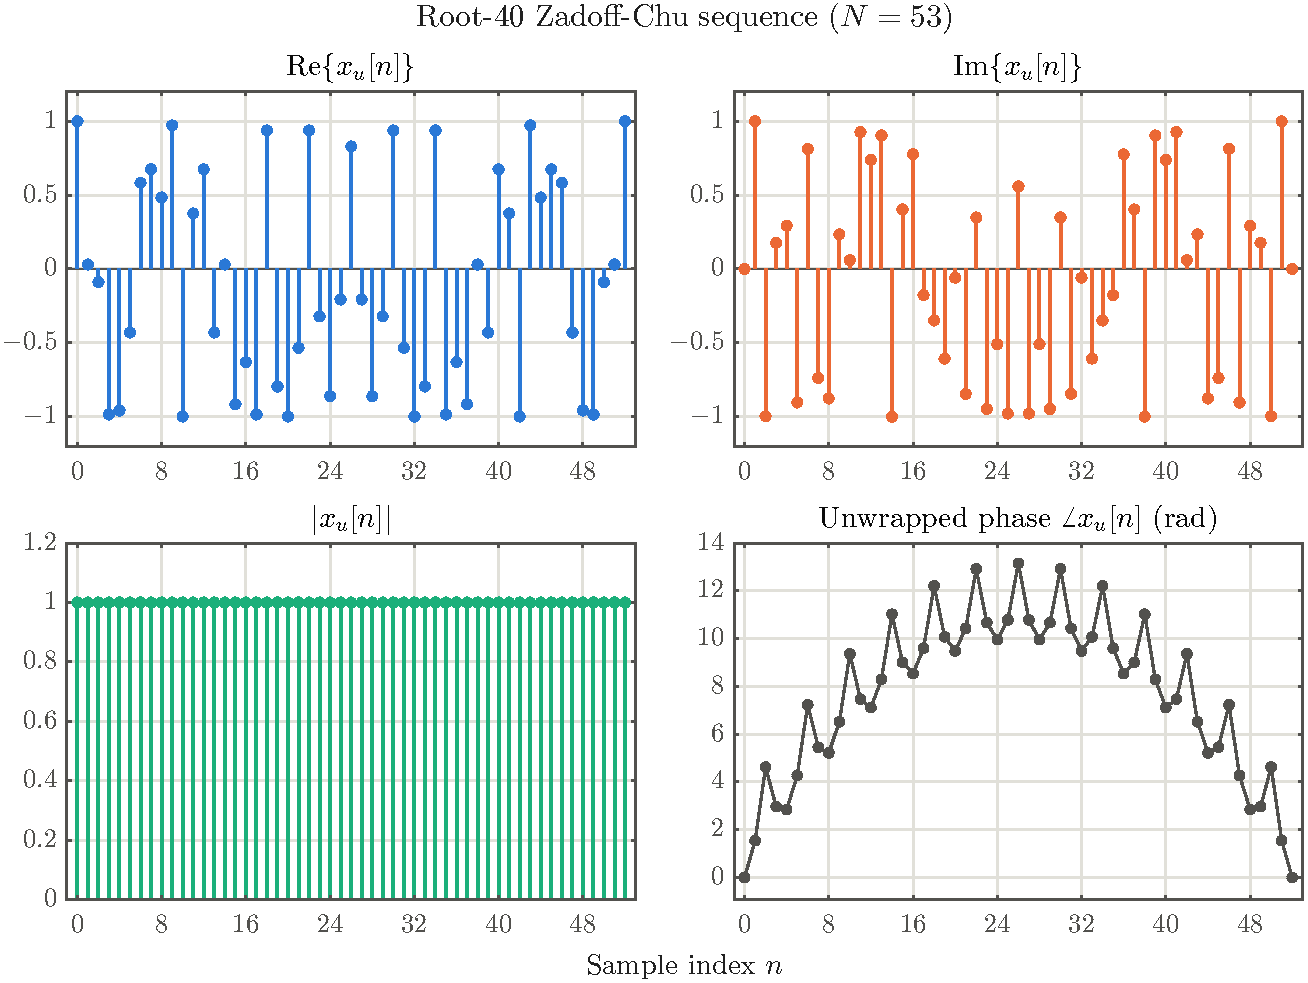
\includegraphics[width=0.95\linewidth]{q1a.pdf}
    \caption{Real Part, Imaginary Part, Magnitude and Unwrapped Phase of $x_{40}[n]$}
\end{figure}

\newpage

\section{(b) Periodic and Linear Autocorrelation}

\question{Calculate and stem-plot the normalized periodic autocorrelation for $l = 0, 1, \ldots, N-1$. (10\%)
Also calculate a nonperiodic linear autocorrelation and explain why it does not exhibit the same zero-sidelobe
property. (10\%)
\[ R_u[l] = \frac{1}{N}\sum_{n=0}^{N-1} x_u[n]\,x_u^*[(n-l) \bmod N], \qquad
   R_u^{\text{lin}}[l] = \frac{1}{N}\sum_{n=l}^{N-1} x_u[n]\,x_u^*[n-l]. \]}

\textbf{Periodic autocorrelation.} The simulation gives $R_u[0] = 1$ and $\max_{l \neq 0}|R_u[l]| = 7.9 \times 10^{-14}$,
which is zero up to the rounding of the large phase arguments. All 52 sidelobes vanish.

\textbf{Why the periodic sidelobes are zero.} The product of a ZC sample with a shifted copy has a phase that is
\emph{linear} in $n$, because the $n^2$ terms cancel:
\begin{equation}
    x_u[n]\,x_u^*[n-l]
    = e^{-j\pi u [\,n(n+1) - (n-l)(n-l+1)\,]/N}
    = \underbrace{e^{-j\pi u(l - l^2)/N}}_{c_l}\; e^{-j2\pi u l n/N}.
\end{equation}
For odd $N$, the same expression also holds with the cyclic index $(n-l) \bmod N$, since replacing $n-l$ by $n-l+N$
changes the phase by $\pi u (2n - 2l + N + 1)$, which is a multiple of $2\pi$. Hence
\begin{equation}
    R_u[l] = \frac{c_l}{N}\sum_{n=0}^{N-1} e^{-j2\pi u l n/N} = c_l\,\delta[l],
\end{equation}
because for $0 < l < N$, $ul$ is not a multiple of the prime $N$, and a complex exponential summed over a whole number
of periods is zero.

\textbf{Linear autocorrelation.} The linear version keeps the same summand but sums only over $n = l, \ldots, N-1$,
i.e.\ $N - l$ terms instead of a full period. The geometric series no longer closes, and
\begin{equation}
    |R_u^{\text{lin}}[l]| = \frac{1}{N}\left|\frac{\sin\big(\pi u l (N-l)/N\big)}{\sin(\pi u l/N)}\right|, \quad l \neq 0 .
\end{equation}
This is nonzero in general. My simulation matches this closed form to $3.9 \times 10^{-14}$ (black circles in the
figure). The largest sidelobe is $|R_u^{\text{lin}}[8]| = 0.1296$ ($-17.7$\,dB) and the mean sidelobe is $0.0278$.

In words: the zero sidelobes come from the cyclic wrap-around. In the periodic case, the samples that fall off the
end of the shifted copy come back at the start, so the product is a complete set of $N$ roots of unity. A linear
correlation drops those $l$ samples, and the remaining partial sum is not zero. This is why LTE adds a cyclic prefix
before the ZC sequence: it makes the receiver's linear correlation look periodic.

\begin{figure}[H]
    \centering
    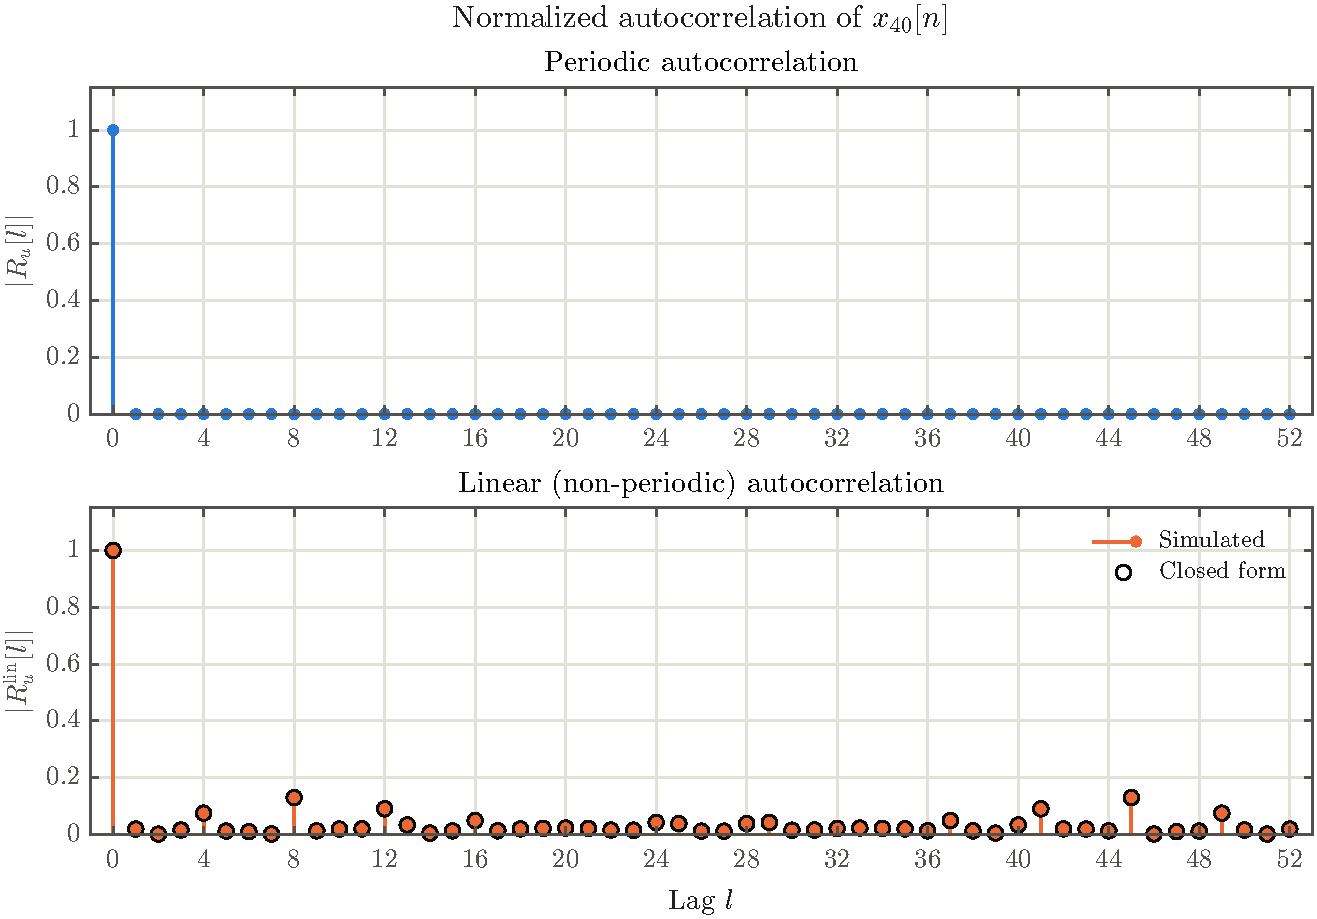
\includegraphics[width=0.92\linewidth]{q1b.pdf}
    \caption{Periodic (top) and Linear (bottom) Autocorrelation of $x_{40}[n]$}
\end{figure}

\newpage

\section{(c) Periodic Cross-Correlation}

\question{Choose $v = 1 + ((u + 16) \bmod 52)$. Calculate the periodic cross-correlation $C_{u,v}[l]$ for
$l = 0, 1, \ldots, N-1$. (10\%)
\[ C_{u,v}[l] = \frac{1}{N}\sum_{n=0}^{N-1} x_u[n]\,x_v^*[(n-l) \bmod N] \]}

With $u = 40$ and $v = 5$, the cross-correlation has the \textbf{same magnitude at every lag}:
\begin{equation}
    |C_{40,5}[l]| = 0.137361 = \frac{1}{\sqrt{53}} \quad \text{for all } l = 0, \ldots, 52,
\end{equation}
with the minimum and maximum equal to six decimals. Only the phase changes with $l$.

The reason is that the $n^2$ terms no longer cancel. The product $x_u[n]x_v^*[n-l]$ has a phase
$-\pi(u - v)n^2/N + (\text{linear in } n)$, so $C_{u,v}[l]$ is a quadratic Gauss sum. For a prime $N$ and
$\gcd(u - v, N) = \gcd(35, 53) = 1$, every such sum has magnitude exactly $\sqrt{N}$, which gives
$|C_{u,v}[l]| = \sqrt{N}/N = 1/\sqrt{N}$. This is the lowest possible flat level for two unit-energy sequences,
because Parseval forces $\sum_l |C_{u,v}[l]|^2 = 1$ (here $53 \times 1/53 = 1$). So two different roots never produce
a false peak: their correlation is spread evenly across all lags.

\begin{figure}[H]
    \centering
    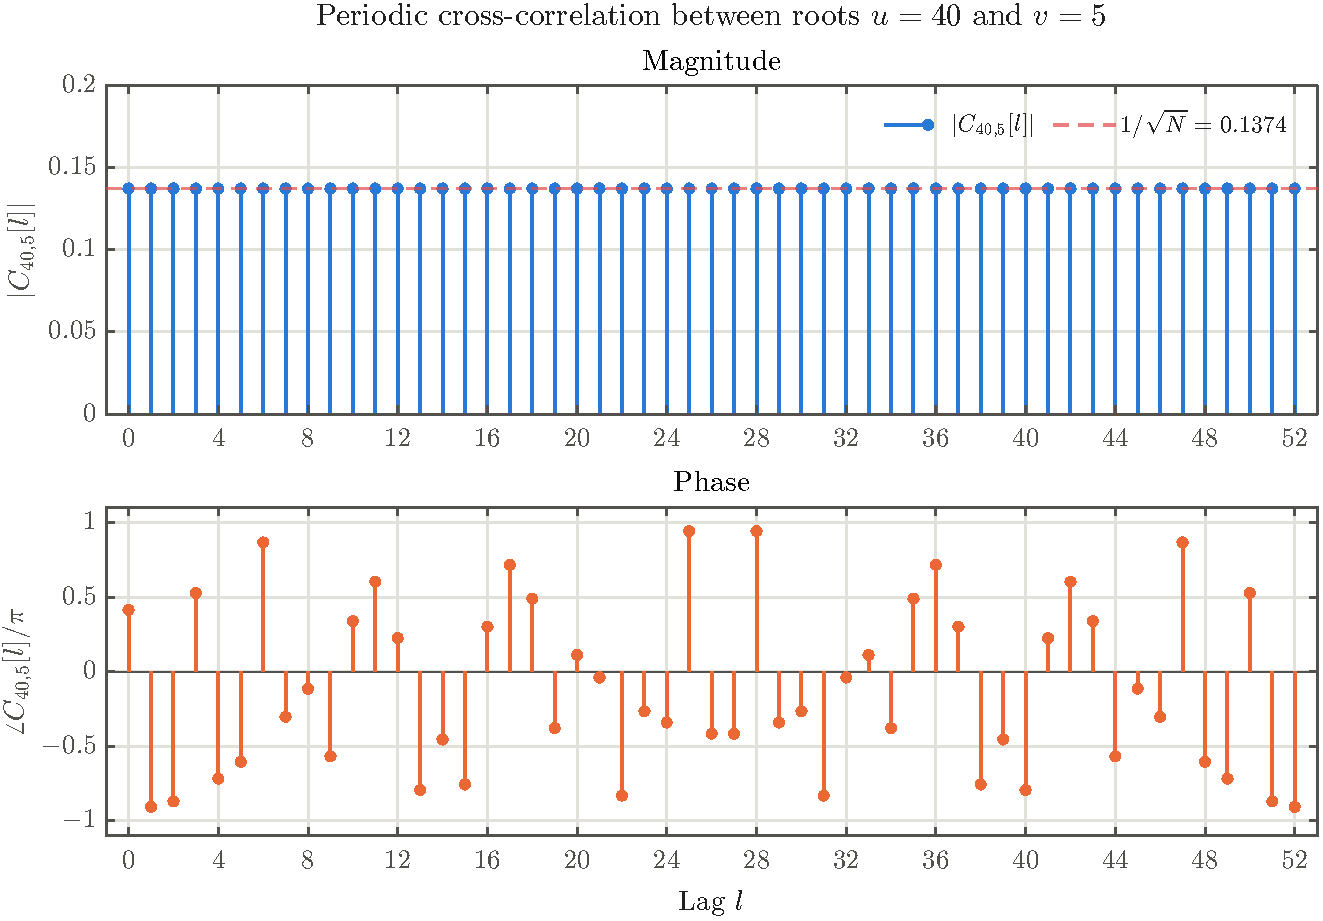
\includegraphics[width=0.92\linewidth]{q1c.pdf}
    \caption{Magnitude (top) and Phase (bottom) of the Periodic Cross-Correlation $C_{40,5}[l]$}
\end{figure}

\newpage

\section{(d) Root and Delay Detection}

\question{Construct a student-specific synchronization test with $u_0 = 3 + ((7m + 2) \bmod 48)$,
$\tau_0 = (5m + 3) \bmod 48$, complex gain $\alpha = \exp(j\pi/5)$. The received signal is defined as
$r[n] = \alpha x_{u_0}[(n - \tau_0) \bmod N]$, $n = 0, 1, \ldots, N-1$. If the set $\Omega = \{u_0 - 2, u_0, u_0 + 2\}$,
search three possible roots in set $\Omega$ and 53 cyclic delays using the metric below. For each root in the set
$\Omega$, draw $D(u, \tau)$ versus $\tau$. (15\%) Report the detected root and delay, and whether they match $u_0$ and
$\tau_0$. Please add some explanations. (5\%)
\[ D(u, \tau) = \left| \frac{1}{N}\sum_{n=0}^{N-1} r[n]\,x_u^*[(n-\tau) \bmod N] \right|
   \quad \text{for } u \in \Omega \text{ and } \tau = 0, 1, \ldots, 52 \]}

With $u_0 = 38$ and $\tau_0 = 6$, the received signal is $r[n] = e^{j\pi/5}\,x_{38}[(n - 6) \bmod 53]$ and the search set
is $\Omega = \{36, 38, 40\}$. I compute all $3 \times 53 = 159$ values of $D(u, \tau)$ and pick the largest.

\begin{table}[H]
\centering
\caption{Detection Metric Summary}
\setlength{\tabcolsep}{12pt}
\renewcommand{\arraystretch}{1.2}
\begin{tabular}{cccc}
\toprule
$u$ & $\max_\tau D(u, \tau)$ & $\arg\max_\tau$ & $D(u, \tau)$ at other lags \\
\midrule
36 & 0.1374 & -- (flat) & 0.1374 at all 53 lags \\
\textbf{38} & \textbf{1.0000} & $\boldsymbol{\tau = 6}$ & 0 (all 52 other lags) \\
40 & 0.1374 & -- (flat) & 0.1374 at all 53 lags \\
\bottomrule
\end{tabular}
\end{table}

\textbf{Result.} The detected pair is $(\hat{u}, \hat{\tau}) = (38, 6)$, which \textbf{matches} $(u_0, \tau_0) = (38, 6)$.
The phase of the correlation at the peak is $0.2000\pi$, so the receiver also recovers $\angle\alpha = \pi/5$
for free.

\textbf{Explanation.} The three curves follow directly from (b) and (c):
\begin{itemize}[leftmargin=1.5em]
    \item \textbf{Correct root ($u = 38$).} $D(u_0, \tau)$ is $|\alpha|$ times the periodic autocorrelation of $x_{38}$
    evaluated at lag $\tau - \tau_0$. By (b) this is $|\alpha| = 1$ at $\tau = \tau_0$ and zero elsewhere, so there is a
    single clean peak and no ambiguity in the delay.
    \item \textbf{Wrong roots ($u = 36, 40$).} $D(u, \tau)$ is a cross-correlation between two different roots. Since
    $u - u_0 = \mp 2$ and $\gcd(2, 53) = 1$, (c) says its magnitude is $1/\sqrt{N} = 0.1374$ at \emph{every} delay.
    The wrong roots give a flat floor rather than a misleading peak (the ``argmax'' of a flat curve is meaningless,
    so I mark it as flat).
    \item \textbf{Margin.} The best wrong candidate is $0.1374$, so the true peak is $7.28\times$ ($17.2$\,dB) above
    anything else. The complex gain does not change this, because $|\alpha| = 1$ scales every value equally and its
    phase disappears inside $|\cdot|$.
\end{itemize}
In a real receiver (for example LTE PSS or PRACH detection), the root identifies the cell or the preamble and the
delay gives the timing. Noise would add a random floor, but with this large margin the decision would stay correct
down to a low SNR.

\begin{figure}[H]
    \centering
    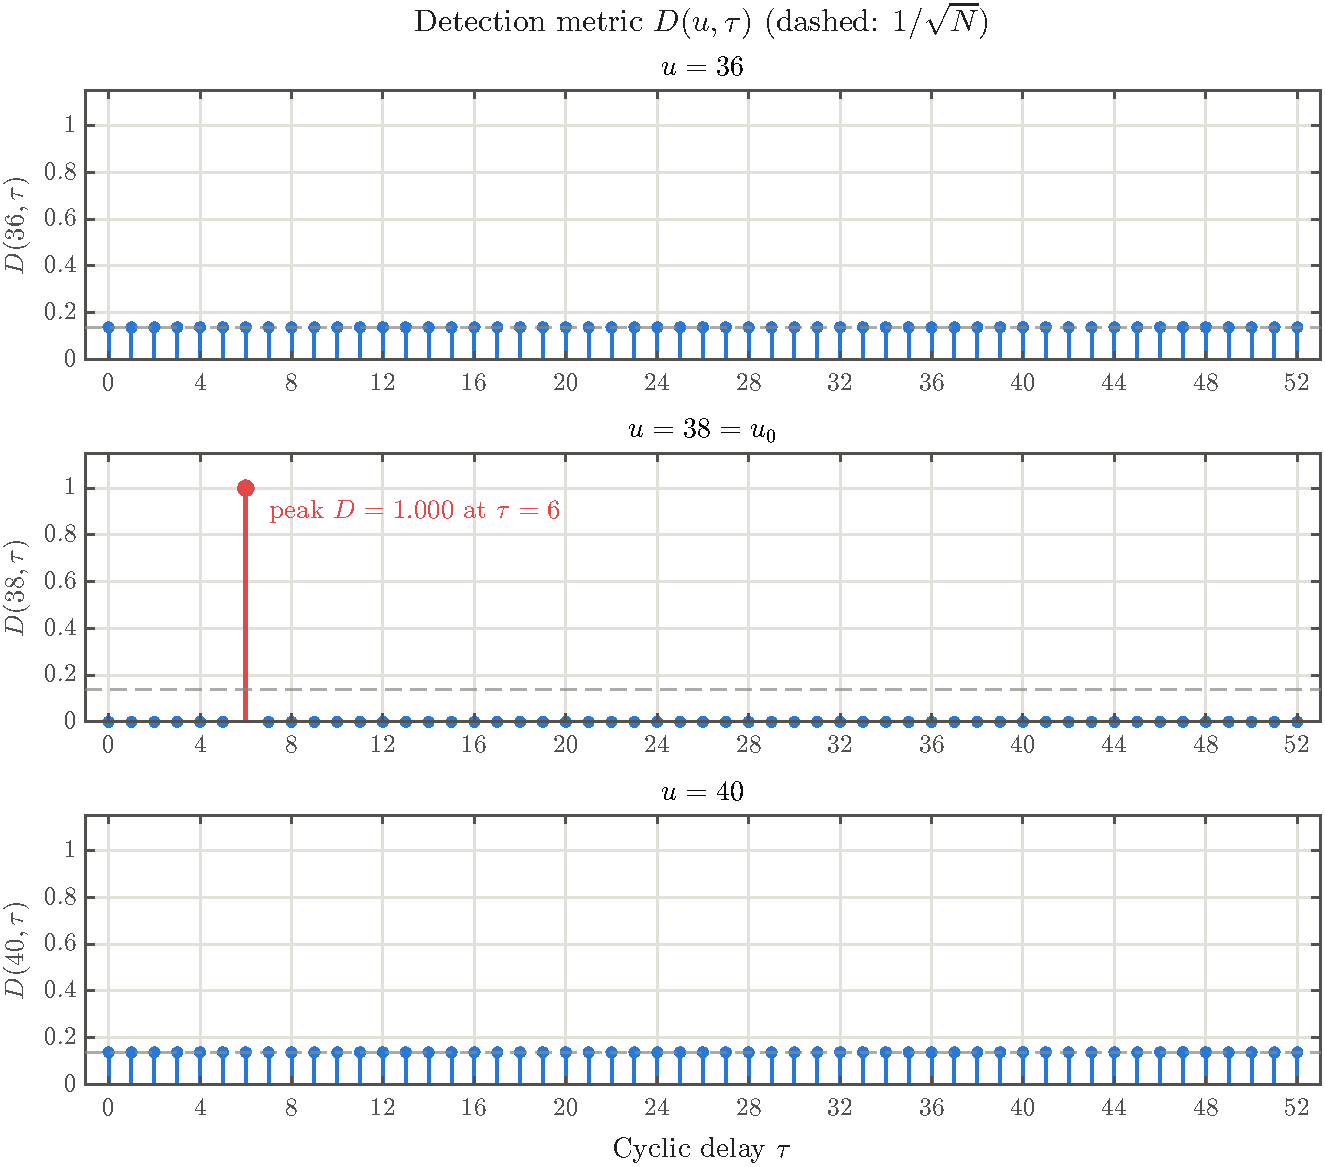
\includegraphics[width=0.88\linewidth]{q1d.pdf}
    \caption{Detection Metric $D(u, \tau)$ for $u = 36$, $38$ and $40$ (red: detected peak)}
\end{figure}

\newpage

% ─────────────────────────────────────────────
\chapter{Q2 — Barker Code Periodic Autocorrelation}
% ─────────────────────────────────────────────
\question{Given the Barker code list in Table 1, please check the periodic autocorrelation function defined as
\[ \Phi_s(k) = \frac{1}{N}\sum_{n=0}^{N-1} S(n)\,S^*((n-k) \bmod N) \]
for $N = 7$ and $13$. (15\%)}

I use the codes exactly as listed in Table~1 of the spec:
\begin{align*}
    N = 7:  &\quad [-1\ -1\ -1\ +1\ +1\ -1\ +1], \\
    N = 13: &\quad [-1\ -1\ -1\ -1\ -1\ +1\ +1\ -1\ -1\ +1\ -1\ +1\ -1].
\end{align*}

\begin{table}[H]
\centering
\caption{$N\Phi_s(k)$ for the Length-7 Barker Code (aperiodic values for reference)}
\setlength{\tabcolsep}{8pt}
\renewcommand{\arraystretch}{1.2}
\begin{tabular}{l*{7}{r}}
\toprule
$k$ & 0 & 1 & 2 & 3 & 4 & 5 & 6 \\
\midrule
$N\Phi_s(k)$ & $7$ & $-1$ & $-1$ & $-1$ & $-1$ & $-1$ & $-1$ \\
Aperiodic $\times N$ & $7$ & $0$ & $-1$ & $0$ & $-1$ & $0$ & $-1$ \\
\bottomrule
\end{tabular}

\end{table}

\begin{table}[H]
\centering
\caption{$N\Phi_s(k)$ for the Length-13 Barker Code (aperiodic values for reference)}
\setlength{\tabcolsep}{5pt}
\renewcommand{\arraystretch}{1.2}
\begin{tabular}{l*{13}{r}}
\toprule
$k$ & 0 & 1 & 2 & 3 & 4 & 5 & 6 & 7 & 8 & 9 & 10 & 11 & 12 \\
\midrule
$N\Phi_s(k)$ & $13$ & $1$ & $1$ & $1$ & $1$ & $1$ & $1$ & $1$ & $1$ & $1$ & $1$ & $1$ & $1$ \\
Aperiodic $\times N$ & $13$ & $0$ & $1$ & $0$ & $1$ & $0$ & $1$ & $0$ & $1$ & $0$ & $1$ & $0$ & $1$ \\
\bottomrule
\end{tabular}

\end{table}

\textbf{Result.} Both periodic autocorrelations are \textbf{two-valued}:
\begin{equation}
    \Phi_s(k) =
    \begin{cases}
        1, & k = 0 \\
        -1/7, & k \neq 0
    \end{cases} \quad (N = 7),
    \qquad
    \Phi_s(k) =
    \begin{cases}
        1, & k = 0 \\
        +1/13, & k \neq 0
    \end{cases} \quad (N = 13).
\end{equation}

\textbf{Why.} A Barker code is defined by its \emph{aperiodic} autocorrelation $A(k) = \sum_{n=k}^{N-1} S(n)S(n-k)$,
whose sidelobes satisfy $|A(k)| \le 1$. For odd $N$, they are $0$ at odd $k$ and $\pm 1$ at even $k$ (second row
of each table). The periodic correlation adds the part that wraps around:
\begin{equation}
    N\Phi_s(k) = A(k) + A(N - k).
\end{equation}
Because $N$ is odd, $k$ and $N - k$ have opposite parity, so exactly one of the two terms is the nonzero $\pm 1$.
That is why every sidelobe has the same value. For $N = 7$ all even-$k$ sidelobes are $-1$, giving $-1/7$; for $N = 13$
they are $+1$, giving $+1/13$.

\textbf{Check by the sum rule.} Summing over all shifts gives $\sum_k N\Phi_s(k) = \big(\sum_n S(n)\big)^2$.
For $N = 7$, $\sum S = -1$, and $7 + 6 \times (-1) = 1 = (-1)^2$. For $N = 13$, $\sum S = -5$, and $13 + 12 \times 1 = 25 = (-5)^2$.
Equivalently, the off-peak value must be $\big((\sum S)^2 - N\big)/\big(N(N-1)\big)$, which the script confirms for both codes.

In short, the Barker codes give a single peak of 1 with flat, tiny sidelobes ($|\Phi_s| = 1/N$) in the periodic sense as
well, which makes them good synchronization words (e.g.\ the 11-chip Barker code in IEEE 802.11b).

\begin{figure}[H]
    \centering
    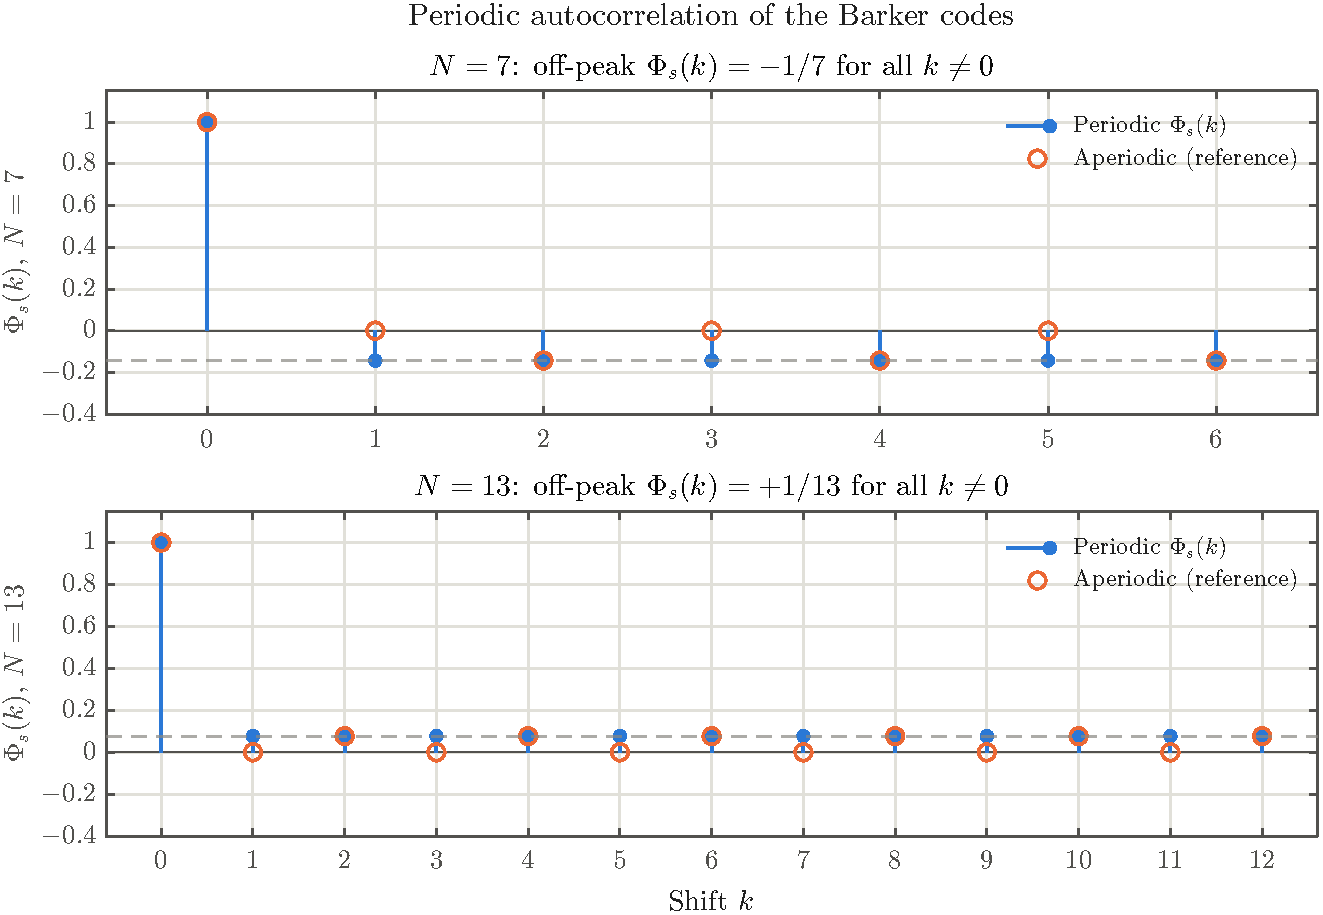
\includegraphics[width=0.92\linewidth]{q2.pdf}
    \caption{Periodic Autocorrelation $\Phi_s(k)$ of the Barker Codes for $N = 7$ (top) and $N = 13$ (bottom); dashed line: off-peak value}
\end{figure}

\newpage

% ─────────────────────────────────────────────
\chapter{Q3 — m-Sequences and Gold Code}
% ─────────────────────────────────────────────
The octal pair $103_8$ and $147_8$ gives
\begin{equation}
    103_8 = (1\,000\,011)_2 \;\Rightarrow\; p(x) = x^6 + x + 1, \qquad
    147_8 = (1\,100\,111)_2 \;\Rightarrow\; p'(x) = x^6 + x^5 + x^2 + x + 1 .
\end{equation}

\textbf{LFSR connection.} I follow the figure in the spec. Each register has six stages numbered 1 (left) to 6 (right).
On every clock, the XOR of the tapped stages enters stage 1, all bits shift one stage to the right, and stage 6 is the
output. Stage $k$ is tapped when $x^k$ appears in the polynomial:
\begin{itemize}[leftmargin=1.5em]
    \item Top LFSR, $p(x) = x^6 + x + 1$: taps at stages \textbf{1 and 6} (the two arrows in the figure).
    \item Bottom LFSR, $p'(x) = x^6 + x^5 + x^2 + x + 1$: taps at stages \textbf{1, 2, 5 and 6} (the four arrows).
\end{itemize}
The Gold generator output is the XOR of the two stage-6 outputs.

\textbf{Initial states.} I write $r_1 = 20$ and $r_2 = 30$ as six-bit binary numbers and load the MSB into stage 1:
$r_1 = 20 \to \texttt{010100}$ and $r_2 = 30 \to \texttt{011110}$. Both are nonzero, as an LFSR needs.

\section{(a) Maximal-Length Sequences}

\question{Set the initial states $r_1$ into the top LFSR and set all 0's as the initial state in the bottom LFSR.
Generate the Maximal-length sequences $s_1[n]$ of 63 bits, for $n = 0, 1, \ldots, 62$. Print the initial values, the
complete sequences. Then, set the initial states $r_2$ into the bottom LFSR and set all 0's as the initial state in the
top LFSR. Generate the Maximal-length sequences $s_2[n]$ of 63 bits, for $n = 0, 1, \ldots, 62$. Print the initial
values, the complete sequences. (10\%)}

An all-zero register stays all zero forever, so in each case the Gold output is just the output of the loaded register
(the script checks that the other register outputs only zeros).

\begin{table}[H]
\centering
\caption{Initial Register Values}
\setlength{\tabcolsep}{14pt}
\renewcommand{\arraystretch}{1.2}
\begin{tabular}{lcc}
\toprule
 & $s_1[n]$ & $s_2[n]$ \\
\midrule
Top LFSR initial state & \texttt{010100} & \texttt{000000} \\
Bottom LFSR initial state & \texttt{000000} & \texttt{011110} \\
\bottomrule
\end{tabular}

\end{table}

\begin{table}[H]
\centering
\caption{Complete m-Sequences $s_1[n]$ and $s_2[n]$ (9 bits per row, $n$ increasing left to right)}
\setlength{\tabcolsep}{14pt}
\renewcommand{\arraystretch}{1.1}
\begin{tabular}{lcc}
\toprule
Sequence & $n$ & Bits \\
\midrule
$s_1[n]$ & 0--8 & \texttt{001010001} \\
 & 9--17 & \texttt{100001000} \\
 & 18--26 & \texttt{001111110} \\
 & 27--35 & \texttt{101011001} \\
 & 36--44 & \texttt{101110110} \\
 & 45--53 & \texttt{100100111} \\
 & 54--62 & \texttt{000101111} \\
\midrule
$s_2[n]$ & 0--8 & \texttt{011110000} \\
 & 9--17 & \texttt{011011100} \\
 & 18--26 & \texttt{110001110} \\
 & 27--35 & \texttt{101111110} \\
 & 36--44 & \texttt{110100010} \\
 & 45--53 & \texttt{000101100} \\
 & 54--62 & \texttt{101010010} \\
\bottomrule
\end{tabular}

\end{table}

\textbf{Checks.} The first six output bits are the initial state read from stage 6 back to stage 1, e.g.\
$s_1[0..5] = \texttt{001010}$ is \texttt{010100} reversed. Both registers visit all $2^6 - 1 = 63$ nonzero states
before returning to the initial state, so the period is exactly 63, which confirms both polynomials are primitive.
Each sequence has 32 ones and 31 zeros (the balance property of an m-sequence).

A note on the convention: with the output at stage 6, the figure's taps produce the recurrence
$s_1[n+6] = s_1[n+5] \oplus s_1[n]$, whose characteristic polynomial is the reciprocal $x^6 + x^5 + 1$ of $p(x)$.
The reciprocal of a primitive polynomial is primitive and just generates the time-reversed m-sequence. Reversing
both sequences only maps a correlation lag $l$ to $-l$, so none of the correlation results below depend on this choice.

\newpage

\section{(b) Periodic Autocorrelation}

\question{Map a binary sequence $s_i[n]$ to $d_i[n] = (-1)^{s_i[n]}$. For both sequences, verify the normalized periodic
autocorrelation for all 63 lags. (20\%)
\[ R_i[l] = \frac{1}{63}\sum_{n=0}^{62} d_i[n]\,d_i[(n+l) \bmod 63] \]}

For both sequences the simulation gives exactly
\begin{equation}
    R_1[l] = R_2[l] =
    \begin{cases}
        1, & l = 0 \\
        -1/63 = -0.0159, & l = 1, \ldots, 62 .
    \end{cases}
\end{equation}
This is the ideal two-valued autocorrelation of an m-sequence. It follows from two properties:
\begin{enumerate}[label=\arabic*)]
    \item \textbf{Shift-and-add.} For $l \neq 0$, $s[n] \oplus s[n+l]$ is another cyclic shift $s[n+k]$ of the same
    m-sequence, because both satisfy the same linear recurrence. In $\pm 1$ form, $d[n]\,d[n+l] = d[n+k]$. The script
    checks this for all 62 nonzero lags of $d_1$.
    \item \textbf{Balance.} Each period has 32 ones and 31 zeros, so $\sum_n d[n] = 31 - 32 = -1$.
\end{enumerate}
Together, $63\,R[l] = \sum_n d[n+k] = -1$ for every $l \neq 0$.

\begin{figure}[H]
    \centering
    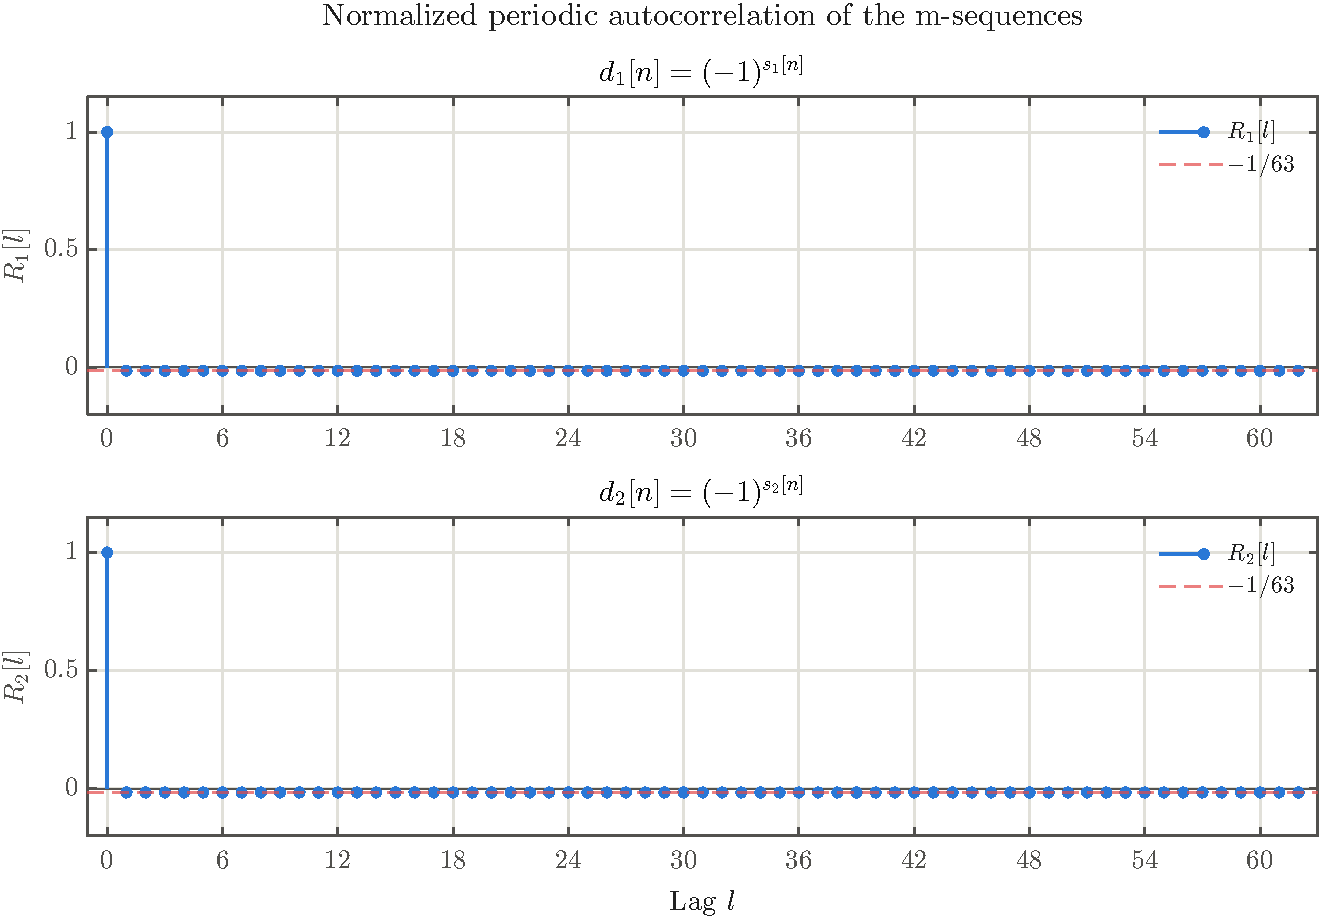
\includegraphics[width=0.92\linewidth]{q3b.pdf}
    \caption{Normalized Periodic Autocorrelation of $d_1[n]$ (top) and $d_2[n]$ (bottom)}
\end{figure}

\newpage

\section{(c) Gold Codeword and Cross-Correlation}

\question{Now, we will construct another codeword of the Gold code. Put initial state $r_1$ and $r_2$ into top LFSR and
bottom LFSR, respectively. Generate the output $s_3[n]$ of 63 bits. Now, map $s_3[n]$ to $d_3[n]$. Then, let's check
the cross-correlation property for $(u, v) = (1, 3)$ and $(u, v) = (2, 3)$ with $N = 63$. (20\%)
\[ C_{u,v}[l] = \frac{1}{N}\sum_{n=0}^{N-1} d_u[n]\,d_v[(n-l) \bmod N] \]}

With top $= \texttt{010100}$ and bottom $= \texttt{011110}$, the Gold generator outputs:

\begin{table}[H]
\centering
\caption{Gold Codeword $s_3[n]$}
\setlength{\tabcolsep}{14pt}
\renewcommand{\arraystretch}{1.1}
\begin{tabular}{lcc}
\toprule
Sequence & $n$ & Bits \\
\midrule
$s_3[n]$ & 0--8 & \texttt{010100001} \\
 & 9--17 & \texttt{111010100} \\
 & 18--26 & \texttt{111110000} \\
 & 27--35 & \texttt{000100111} \\
 & 36--44 & \texttt{011010100} \\
 & 45--53 & \texttt{100001011} \\
 & 54--62 & \texttt{101111101} \\
\bottomrule
\end{tabular}

\end{table}

The two registers do not interact, so $s_3[n] = s_1[n] \oplus s_2[n]$ (confirmed bit by bit), and in $\pm 1$ form
$d_3[n] = d_1[n]\,d_2[n]$.

The cross-correlations take \textbf{only three values}:

\begin{table}[H]
\centering
\caption{Values of $63\,C_{u,v}[l]$ over All 63 Lags}
\setlength{\tabcolsep}{14pt}
\renewcommand{\arraystretch}{1.2}
\begin{tabular}{lccc|c}
\toprule
 & $-17$ & $-1$ & $15$ & $\max_l |C_{u,v}[l]|$ \\
\midrule
$C_{1,3}$ & 6 & 47 & 10 & $17/63 = 0.2698$ \\
$C_{2,3}$ & 6 & 47 & 10 & $17/63 = 0.2698$ \\
\bottomrule
\end{tabular}
\end{table}

So $C_{1,3}[l], C_{2,3}[l] \in \{-17/63,\ -1/63,\ 15/63\}$, and the largest magnitude is $17/63 = 0.27$, far below the
autocorrelation peak of 1.

\begin{figure}[H]
    \centering
    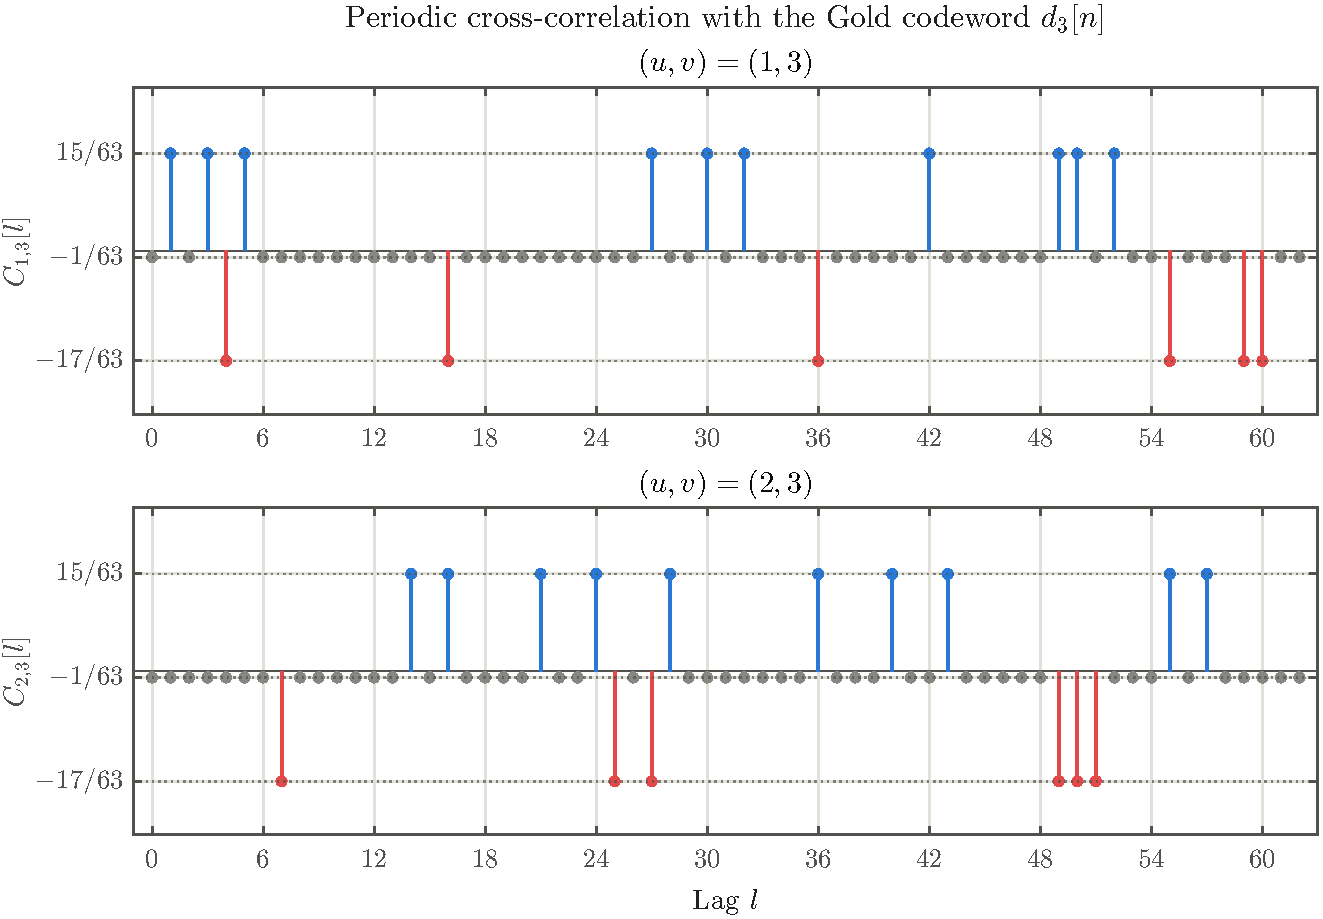
\includegraphics[width=0.92\linewidth]{q3c.pdf}
    \caption{Periodic Cross-Correlation $C_{1,3}[l]$ (top) and $C_{2,3}[l]$ (bottom); blue: $15/63$, gray: $-1/63$, red: $-17/63$}
\end{figure}

\newpage

\section{(d) Is the Answer in (c) Correct?}

\question{Please judge if your answer in (c) is correct or not? Please state the reason. (5\%)}

\textbf{Yes, the answer in (c) is correct.} The reasons are:

\textbf{1) It matches Gold's theorem.} $p(x)$ and $p'(x)$ are a preferred pair of degree $n = 6$. For a preferred pair,
the periodic cross-correlation of the two m-sequences, and of any two codewords in the Gold family they generate,
takes only the three values
\begin{equation}
    \frac{1}{N}\left\{-t(n),\ -1,\ t(n) - 2\right\}, \qquad
    t(n) = 1 + 2^{\lfloor (n+2)/2 \rfloor} = 1 + 2^{4} = 17 ,
\end{equation}
i.e.\ $\{-17, -1, 15\}/63$. This is exactly the set I get for $C_{1,3}$ and $C_{2,3}$.

\textbf{2) The value counts also match.} I can show $C_{1,3}$ must behave like $C_{1,2}$. Using $d_3 = d_1 d_2$,
\begin{equation}
    63\,C_{1,3}[l] = \sum_n \underbrace{d_1[n]\,d_1[n-l]}_{=\,d_1[n-k] \text{ for } l \neq 0}\, d_2[n-l],
\end{equation}
so for $l \neq 0$ it is the cross-correlation of $d_1$ and $d_2$ at another lag, and at $l = 0$ it equals
$\sum_n d_2[n] = -1$. The same argument works for $C_{2,3}$. For a preferred pair with $n = 6$ (decimation
$q = 2^k + 1 = 5$, $e = \gcd(n, k) = 2$), theory gives how often each value occurs:
\begin{equation}
    -17\!: 2^{n-e-1} - 2^{\frac{n-e}{2}-1} = 6, \qquad
    -1\!: 2^{n} - 2^{n-e} - 1 = 47, \qquad
    15\!: 2^{n-e-1} + 2^{\frac{n-e}{2}-1} = 10 .
\end{equation}
My $C_{1,2}$, $C_{1,3}$ and $C_{2,3}$ all show exactly 6, 47 and 10 (see the figure below).

\textbf{3) The pair really is preferred.} Taking every fifth bit of $s_1$, $s_1[5n \bmod 63]$, gives $s_2$ shifted by
6 lags, so $s_2$ is the $q = 5$ decimation of $s_1$. Gold's condition holds: $q = 2^2 + 1$ and $n/\gcd(n, 2) = 3$ is odd.
(Other values such as $q = 13, 21, 23$ do not give $s_2$.)

\textbf{4) Sum check.} For any two $\pm 1$ sequences, $\sum_l C_{u,v}[l] = \frac{1}{N}\big(\sum_n d_u[n]\big)\big(\sum_n d_v[n]\big)$.
All three sequences have 32 ones, so each sum is $(-1)(-1)/63 = 1/63$. From the table:
$(6 \times (-17) + 47 \times (-1) + 10 \times 15)/63 = 1/63$. \checkmark

\textbf{5) Brute force over the whole family.} The Gold family has $N + 2 = 65$ codewords: $d_1$, $d_2$ and
$d_1[n]\,d_2[n+k]$ for $k = 0, \ldots, 62$. Checking all $\binom{65}{2} = 2080$ pairs at all 63 lags, the
cross-correlation never leaves $\{-17, -1, 15\}/63$.

One more remark: $d_3$ itself is not an m-sequence, so its autocorrelation is not two-valued. Its 62 sidelobes take the
values $-17$, $-1$ and $15$ (over 63) as well, 12, 38 and 12 times. This is the price of the Gold family: it trades the ideal
$-1/63$ autocorrelation of an m-sequence for 65 codewords with a guaranteed low cross-correlation of at most $17/63$,
which is what a CDMA system such as GPS needs to separate many users.

\begin{figure}[H]
    \centering
    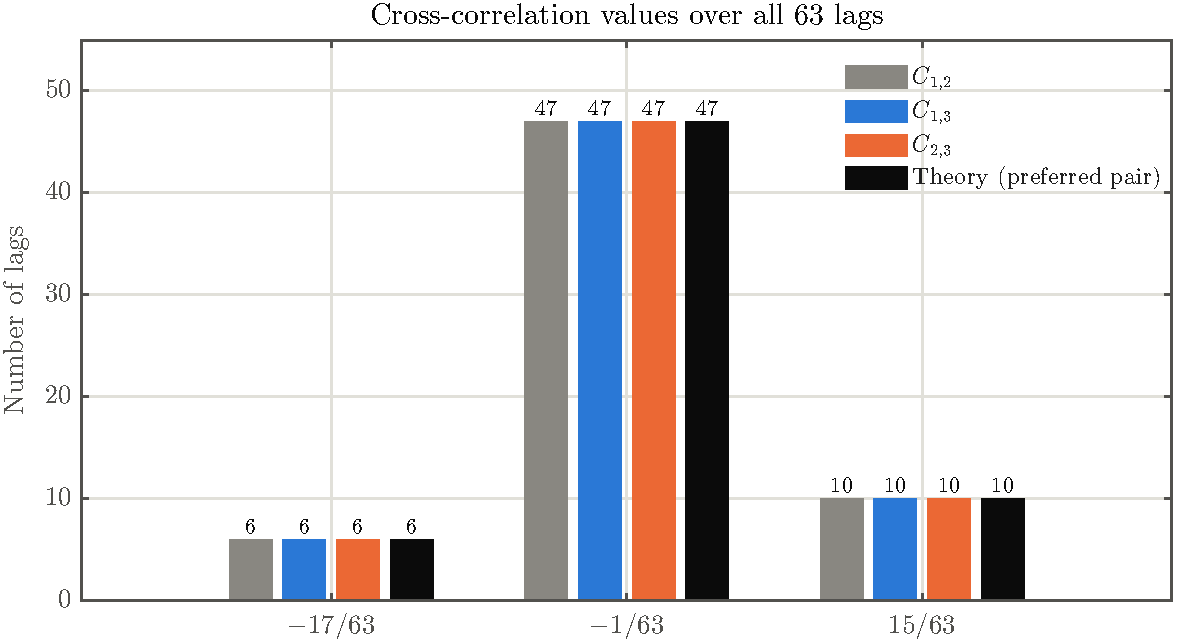
\includegraphics[width=0.9\linewidth]{q3d.pdf}
    \caption{Number of Lags at Each Cross-Correlation Value Compared with the Preferred-Pair Theory}
\end{figure}

\newpage

% ─────────────────────────────────────────────
\chapter{AI Tool Disclosure}
\label{ch:ai}
% ─────────────────────────────────────────────
\question{Please disclose how you use AI tools and its version.}

I used \textbf{Claude Opus 5.5} to help with this homework in the following four parts:
\begin{enumerate}[label=(\arabic*)]
    \item Understanding the homework specification.
    \item Assisting with the MATLAB code.
    \item Plotting the figures.
    \item Writing this \LaTeX{} report.
\end{enumerate}

\end{document}
